\documentclass{article}
\usepackage[T1]{fontenc}
\usepackage{lmodern}
\usepackage{graphicx}
\usepackage{amsmath,amssymb}
\usepackage[a4paper,margin=2cm]{geometry}
\usepackage[absolute,overlay]{textpos}
\setlength{\TPHorizModule}{1mm}
\setlength{\TPVertModule}{1mm}
\usepackage[indonesian]{babel}
\usepackage{hyperref}
\setlength{\emergencystretch}{2em}
% unit: Halaman 50

\begin{document}

% === Halaman 50 (llm) ===

\section*{Keamanan ECC}

\vspace{133.65mm}

\begin{itemize}
    \item Untuk mengenkripsi kunci AES-128 dengan algoritma kriptografi kunci public, maka:
    \begin{itemize}
        \item Ukuran kunci RSA: 3072 bit
        \item Ukuran kunci ECC cuku 256 bit saja
    \end{itemize}
    \vspace{10mm}
    \item Bagaimana cara meningkatkan keamanan RSA?
    \begin{itemize}
        \item Tingkatkan ukuran kunci
        \item \textcolor{red}{Tidak Praktis?}
    \end{itemize}
    \item Dengan ECC, pertambahan ukuran kunci tidak signifikan dibandingkan RSA
\end{itemize}

\vspace{5mm}
\begin{flushright}
\small *) Sumber bahan: \textcolor{red}{Debdeep Mukhopadhyay, Elliptic Curve Cryptography}, \textcolor{red}{Dept of Computer Sc and Engg IIT Madras}
\end{flushright}

% deskripsi: Tabel pedoman NIST untuk perbandingan ukuran kunci public (ECC dan RSA) terhadap ukuran kunci AES.
% bbox normalisasi: [0.5300, 0.2800, 0.9400, 0.7300]
\begin{textblock*}{86.10mm}(111.30mm,83.16mm)
\noindent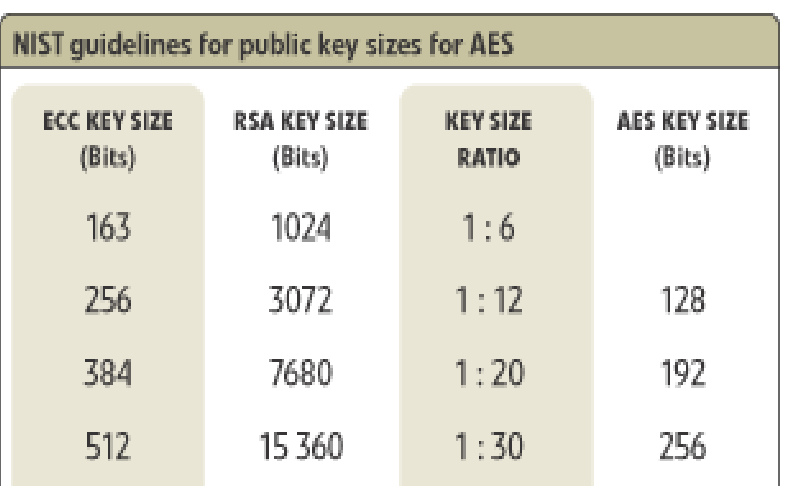
\includegraphics[width=86.10mm,height=133.65mm]{../../images/llm/page_050_img_01.png}%
\end{textblock*}

\end{document}
